% Created by tikzDevice version 0.12.6 on 2024-03-15 15:16:48
% !TEX encoding = UTF-8 Unicode
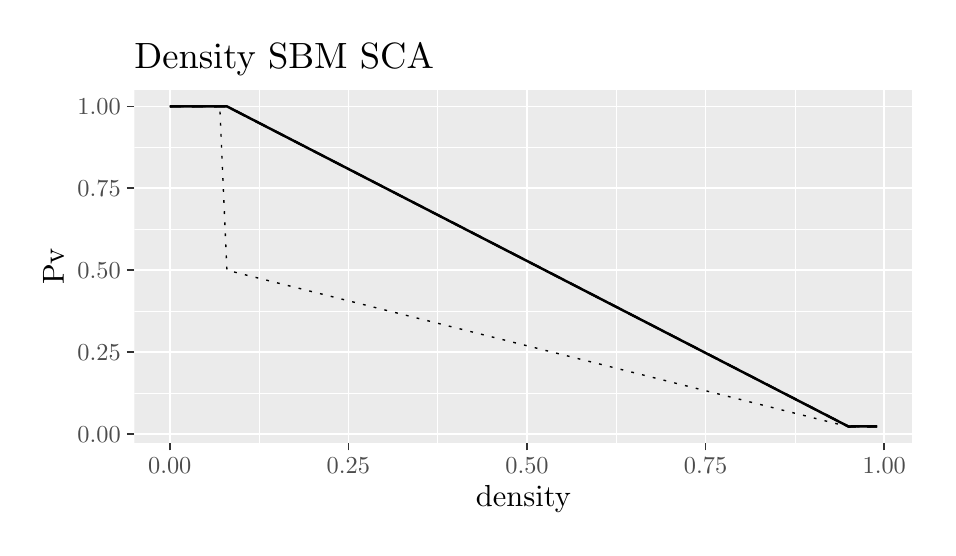
\begin{tikzpicture}[x=1pt,y=1pt]
\definecolor{fillColor}{RGB}{255,255,255}
\path[use as bounding box,fill=fillColor,fill opacity=0.00] (0,0) rectangle (325.21,180.67);
\begin{scope}
\path[clip] (  0.00,  0.00) rectangle (325.21,180.67);
\definecolor{drawColor}{RGB}{255,255,255}
\definecolor{fillColor}{RGB}{255,255,255}

\path[draw=drawColor,line width= 0.6pt,line join=round,line cap=round,fill=fillColor] (  0.00,  0.00) rectangle (325.21,180.68);
\end{scope}
\begin{scope}
\path[clip] ( 38.56, 30.69) rectangle (319.71,158.02);
\definecolor{fillColor}{gray}{0.92}

\path[fill=fillColor] ( 38.56, 30.69) rectangle (319.71,158.02);
\definecolor{drawColor}{RGB}{255,255,255}

\path[draw=drawColor,line width= 0.3pt,line join=round] ( 38.56, 48.64) --
	(319.71, 48.64);

\path[draw=drawColor,line width= 0.3pt,line join=round] ( 38.56, 78.24) --
	(319.71, 78.24);

\path[draw=drawColor,line width= 0.3pt,line join=round] ( 38.56,107.83) --
	(319.71,107.83);

\path[draw=drawColor,line width= 0.3pt,line join=round] ( 38.56,137.43) --
	(319.71,137.43);

\path[draw=drawColor,line width= 0.3pt,line join=round] ( 83.61, 30.69) --
	( 83.61,158.02);

\path[draw=drawColor,line width= 0.3pt,line join=round] (148.15, 30.69) --
	(148.15,158.02);

\path[draw=drawColor,line width= 0.3pt,line join=round] (212.70, 30.69) --
	(212.70,158.02);

\path[draw=drawColor,line width= 0.3pt,line join=round] (277.24, 30.69) --
	(277.24,158.02);

\path[draw=drawColor,line width= 0.6pt,line join=round] ( 38.56, 33.84) --
	(319.71, 33.84);

\path[draw=drawColor,line width= 0.6pt,line join=round] ( 38.56, 63.44) --
	(319.71, 63.44);

\path[draw=drawColor,line width= 0.6pt,line join=round] ( 38.56, 93.04) --
	(319.71, 93.04);

\path[draw=drawColor,line width= 0.6pt,line join=round] ( 38.56,122.63) --
	(319.71,122.63);

\path[draw=drawColor,line width= 0.6pt,line join=round] ( 38.56,152.23) --
	(319.71,152.23);

\path[draw=drawColor,line width= 0.6pt,line join=round] ( 51.34, 30.69) --
	( 51.34,158.02);

\path[draw=drawColor,line width= 0.6pt,line join=round] (115.88, 30.69) --
	(115.88,158.02);

\path[draw=drawColor,line width= 0.6pt,line join=round] (180.43, 30.69) --
	(180.43,158.02);

\path[draw=drawColor,line width= 0.6pt,line join=round] (244.97, 30.69) --
	(244.97,158.02);

\path[draw=drawColor,line width= 0.6pt,line join=round] (309.52, 30.69) --
	(309.52,158.02);
\definecolor{drawColor}{RGB}{0,0,0}

\path[draw=drawColor,line width= 0.9pt,line join=round] ( 51.34,152.23) --
	( 53.92,152.23) --
	( 56.50,152.23) --
	( 59.08,152.23) --
	( 61.66,152.23) --
	( 64.24,152.23) --
	( 66.83,152.23) --
	( 69.41,152.23) --
	( 71.99,152.23) --
	(296.61, 36.53) --
	(299.19, 36.60) --
	(301.77, 36.60) --
	(304.35, 36.60) --
	(306.94, 36.60);

\path[draw=drawColor,line width= 0.7pt,dash pattern=on 4pt off 4pt ,line join=round] ( 51.34,152.23) --
	( 53.92,152.23) --
	( 56.50,152.23) --
	( 59.08,152.23) --
	( 61.66,152.23) --
	( 64.24,152.23) --
	( 66.83,152.23) --
	( 69.41,152.23) --
	( 71.99,152.23) --
	(296.61, 36.53) --
	(299.19, 36.53) --
	(301.77, 36.53) --
	(304.35, 36.53) --
	(306.94, 36.53);

\path[draw=drawColor,line width= 0.7pt,dash pattern=on 4pt off 4pt ,line join=round] ( 51.34,152.23) --
	( 53.92,152.23) --
	( 56.50,152.23) --
	( 59.08,152.23) --
	( 61.66,152.23) --
	( 64.24,152.23) --
	( 66.83,152.23) --
	( 69.41,152.23) --
	( 71.99,152.23) --
	(296.61, 36.60) --
	(299.19, 36.60) --
	(301.77, 36.60) --
	(304.35, 36.60) --
	(306.94, 36.60);

\path[draw=drawColor,line width= 0.5pt,dash pattern=on 1pt off 3pt ,line join=round] ( 51.34,152.23) --
	( 53.92,152.23) --
	( 56.50,152.23) --
	( 59.08,152.23) --
	( 61.66,152.23) --
	( 64.24,152.23) --
	( 66.83,152.23) --
	( 69.41,152.23) --
	( 71.99, 93.04) --
	(296.61, 36.47) --
	(299.19, 36.53) --
	(301.77, 36.53) --
	(304.35, 36.53) --
	(306.94, 36.53);

\path[draw=drawColor,line width= 0.5pt,dash pattern=on 1pt off 3pt ,line join=round] ( 51.34,152.23) --
	( 53.92,152.23) --
	( 56.50,152.23) --
	( 59.08,152.23) --
	( 61.66,152.23) --
	( 64.24,152.23) --
	( 66.83,152.23) --
	( 69.41,152.23) --
	( 71.99,152.23) --
	(296.61, 36.60) --
	(299.19, 36.60) --
	(301.77, 36.60) --
	(304.35, 36.60) --
	(306.94, 36.60);
\end{scope}
\begin{scope}
\path[clip] (  0.00,  0.00) rectangle (325.21,180.67);
\definecolor{drawColor}{gray}{0.30}

\node[text=drawColor,anchor=base east,inner sep=0pt, outer sep=0pt, scale=  0.88] at ( 33.61, 30.81) {0.00};

\node[text=drawColor,anchor=base east,inner sep=0pt, outer sep=0pt, scale=  0.88] at ( 33.61, 60.41) {0.25};

\node[text=drawColor,anchor=base east,inner sep=0pt, outer sep=0pt, scale=  0.88] at ( 33.61, 90.01) {0.50};

\node[text=drawColor,anchor=base east,inner sep=0pt, outer sep=0pt, scale=  0.88] at ( 33.61,119.60) {0.75};

\node[text=drawColor,anchor=base east,inner sep=0pt, outer sep=0pt, scale=  0.88] at ( 33.61,149.20) {1.00};
\end{scope}
\begin{scope}
\path[clip] (  0.00,  0.00) rectangle (325.21,180.67);
\definecolor{drawColor}{gray}{0.20}

\path[draw=drawColor,line width= 0.6pt,line join=round] ( 35.81, 33.84) --
	( 38.56, 33.84);

\path[draw=drawColor,line width= 0.6pt,line join=round] ( 35.81, 63.44) --
	( 38.56, 63.44);

\path[draw=drawColor,line width= 0.6pt,line join=round] ( 35.81, 93.04) --
	( 38.56, 93.04);

\path[draw=drawColor,line width= 0.6pt,line join=round] ( 35.81,122.63) --
	( 38.56,122.63);

\path[draw=drawColor,line width= 0.6pt,line join=round] ( 35.81,152.23) --
	( 38.56,152.23);
\end{scope}
\begin{scope}
\path[clip] (  0.00,  0.00) rectangle (325.21,180.67);
\definecolor{drawColor}{gray}{0.20}

\path[draw=drawColor,line width= 0.6pt,line join=round] ( 51.34, 27.94) --
	( 51.34, 30.69);

\path[draw=drawColor,line width= 0.6pt,line join=round] (115.88, 27.94) --
	(115.88, 30.69);

\path[draw=drawColor,line width= 0.6pt,line join=round] (180.43, 27.94) --
	(180.43, 30.69);

\path[draw=drawColor,line width= 0.6pt,line join=round] (244.97, 27.94) --
	(244.97, 30.69);

\path[draw=drawColor,line width= 0.6pt,line join=round] (309.52, 27.94) --
	(309.52, 30.69);
\end{scope}
\begin{scope}
\path[clip] (  0.00,  0.00) rectangle (325.21,180.67);
\definecolor{drawColor}{gray}{0.30}

\node[text=drawColor,anchor=base,inner sep=0pt, outer sep=0pt, scale=  0.88] at ( 51.34, 19.68) {0.00};

\node[text=drawColor,anchor=base,inner sep=0pt, outer sep=0pt, scale=  0.88] at (115.88, 19.68) {0.25};

\node[text=drawColor,anchor=base,inner sep=0pt, outer sep=0pt, scale=  0.88] at (180.43, 19.68) {0.50};

\node[text=drawColor,anchor=base,inner sep=0pt, outer sep=0pt, scale=  0.88] at (244.97, 19.68) {0.75};

\node[text=drawColor,anchor=base,inner sep=0pt, outer sep=0pt, scale=  0.88] at (309.52, 19.68) {1.00};
\end{scope}
\begin{scope}
\path[clip] (  0.00,  0.00) rectangle (325.21,180.67);
\definecolor{drawColor}{RGB}{0,0,0}

\node[text=drawColor,anchor=base,inner sep=0pt, outer sep=0pt, scale=  1.10] at (179.14,  7.64) {density};
\end{scope}
\begin{scope}
\path[clip] (  0.00,  0.00) rectangle (325.21,180.67);
\definecolor{drawColor}{RGB}{0,0,0}

\node[text=drawColor,rotate= 90.00,anchor=base,inner sep=0pt, outer sep=0pt, scale=  1.10] at ( 13.08, 94.35) {Pv};
\end{scope}
\begin{scope}
\path[clip] (  0.00,  0.00) rectangle (325.21,180.67);
\definecolor{drawColor}{RGB}{0,0,0}

\node[text=drawColor,anchor=base west,inner sep=0pt, outer sep=0pt, scale=  1.32] at ( 38.56,166.08) {Density SBM SCA};
\end{scope}
\end{tikzpicture}
